% \title{Apunte de Matemáticas Discretas CC3101:\\ 
% Caminos,  circuitos eulerianos y hamiltonianos  Clase 19}
% % \title{Ejercicios Lógica e Inducción}
% \author{Andrés Abeliuk}
% \date{}
% \maketitle


\section{Circuitos Eulerianos}

\subsection{El Problema de los Puentes de Königsberg}

En el siglo XVIII, en la ciudad prusiana de Königsberg, se planteó una pregunta curiosa sobre la posibilidad de recorrer la ciudad cruzando todos sus puentes exactamente una vez. La ciudad estaba dividida por el río Pregel en cuatro regiones conectadas por siete puentes.

\begin{center}
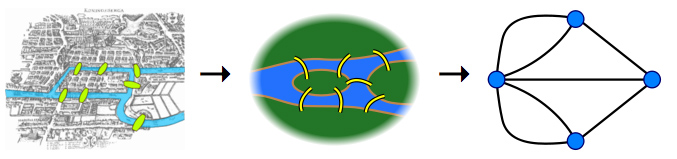
\includegraphics[width=0.9\textwidth]{Figures/bridges.jpg} \\
\smallskip
\small{\textit{Abstracción del problema de los Puentes de Königsberg: desde el mapa original hasta su representación como grafo.}} \
\href{https://en.wikipedia.org/wiki/File:Konigsberg_bridges.png}{\scriptsize{Imagen: Bogdan Giuşcă.}}
\end{center}

\begin{quote}
\textbf{Problema:} ¿Es posible comenzar en una región cualquiera, recorrer todos los puentes exactamente una vez, y volver al punto de partida?
\end{quote}

Este problema intrigó a los matemáticos de la época, y fue Leonhard Euler quien, en 1736, ofreció una solución formal, dando origen a la teoría de grafos.

\subsection{Modelado con Grafos}

Podemos modelar este problema mediante un \textbf{grafo}, donde cada región se representa con un vértice y cada puente con una arista que conecta dos vértices.

\begin{center}
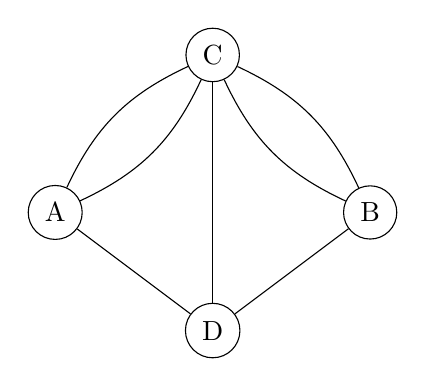
\begin{tikzpicture}[scale=1, every node/.style={circle, draw}]
  \node (A) at (0,0) {A};
  \node (B) at (4,0) {B};
  \node (C) at (2,2) {C};
  \node (D) at (2,-1.5) {D};

  \draw (A) to[bend left=20] (C);
  \draw (A) to[bend right=20] (C);
  \draw (B) to[bend left=20] (C);
  \draw (B) to[bend right=20] (C);
  \draw (D) -- (C);
  \draw (A) -- (D);
  \draw (B) -- (D);
\end{tikzpicture}
\end{center}

El problema se convierte ahora en determinar si existe un \textbf{circuito euleriano} en este grafo.

\medskip

\begin{definitionblock}{Definición: Circuito Euleriano}
Sea $G$ un grafo. Un \emph{circuito euleriano} es un circuito simple que recorre cada arista de $G$ exactamente una vez.
\end{definitionblock}

\begin{exampleblock}{Ejemplo}
El siguiente grafo posee múltiples circuitos eulerianos:

\begin{center}
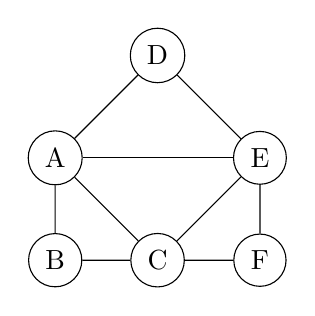
\begin{tikzpicture}[scale=1.3, every node/.style={circle, draw, fill=white, minimum size=6mm}]
  \node (A) at (-1,0) {A};
  \node (B) at (-1,-1) {B};
  \node (C) at (0,-1) {C};
  \node (F) at (1,-1) {F};
  \node (E) at (1,0) {E};
  \node (D) at (0,1) {D};

  \draw (A) -- (B);
  \draw (A) -- (C);
  \draw (A) -- (D);
  \draw (A) -- (E);
  \draw (B) -- (C);
  \draw (C) -- (F);
  \draw (C) -- (E);
  \draw (E) -- (F);
  \draw (D) -- (E);
\end{tikzpicture}
\end{center}

Algunos circuitos eulerianos posibles (empezando en $A$) son:
\[
ADEACEFCBA \quad \text{y} \quad AECABCFEDA
\]
\end{exampleblock}

\begin{thmblock}{Teorema Clásico de Euler}
Un multigrafo conexo tiene un circuito euleriano si y sólo si todos sus vértices tienen grado par.
\end{thmblock}

\subsection{Solución al problema de los puentes de Königsberg}

El problema de los puentes de Königsberg no tiene solución: el grafo que lo representa tiene cuatro vértices de grado impar, lo cual impide la existencia de un circuito euleriano. Este resultado marcó el inicio del estudio sistemático de grafos, un área fundamental en la matemática discreta y la informática.

\subsection{Demostración del Teorema de Euler}

\textbf{($\Rightarrow$)} Supongamos que $G$ tiene un circuito euleriano. Cada vez que el circuito pasa por un vértice, debe entrar y luego salir por aristas distintas, lo que contribuye con dos al grado de ese vértice. Como el circuito pasa por todas las aristas del grafo (por definición), y $G$ es conexo, todos los vértices deben tener grado par.

\medskip

\textbf{($\Leftarrow$)} Supongamos ahora que $G$ es conexo y que todos sus vértices tienen grado par. Construiremos un circuito euleriano de forma constructiva:

\begin{itemize}
  \item Elegimos un vértice cualquiera \( v_0 \) y un arco \( (v_0, v_1) \) incidente.
  \item Continuamos extendiendo un camino \( v_0, v_1, v_2, \dots, v_n \) de forma que no repita aristas y se detenga sólo cuando no sea posible continuar.
\end{itemize}

\begin{thmblock}{Proposición}
En el procedimiento anterior, necesariamente se cumple \( v_0 = v_n \), es decir, se obtiene un circuito.
\end{thmblock}

\begin{proof}
Supongamos lo contrario: que \( v_0 \neq v_n \). Entonces el camino termina en un vértice \( v_n \) con grado impar (ya que entró una sola vez). Pero esto contradice la hipótesis de que todos los vértices tienen grado par. Por lo tanto, el circuito debe cerrar.
\end{proof}

Por lo tanto tenemos un circuito simple 
$$v_0, v_1, v_2, \dots, v_{n-1}, v_0$$
Si el circuito contiene todos los arcos, la prueba está
terminada. 
% Si no, construimos un subgrafo $G'$ de $G$ borrando todos los arcos del circuito.
Si no, eliminamos sus aristas del grafo \( G \) y obtenemos un subgrafo \( G' \) con vértices de grado par (aunque $G'$ puede ser disconexo). Como \( G \) es conexo, existe al menos un vértice, $v'$, en común entre \( G' \) y el circuito original. A partir de dicho vértice se puede construir un nuevo circuito en \( G' \) y componerlo con el anterior.



\begin{center}
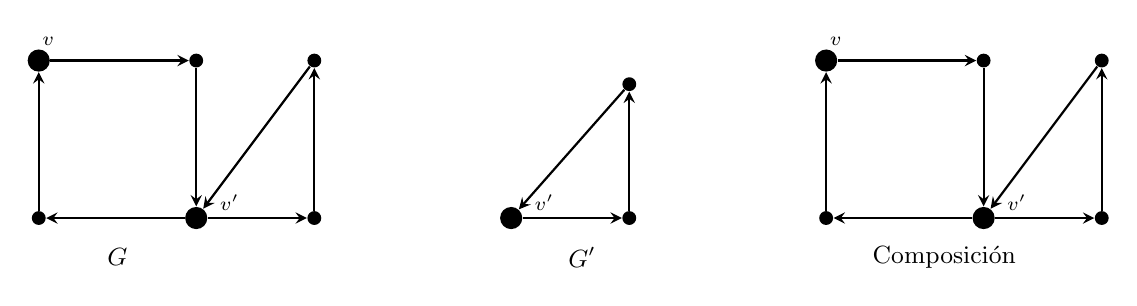
\begin{tikzpicture}[
  scale=1,
  vtx/.style={circle, fill=black, inner sep=0pt, minimum size=5pt},
  hvtx/.style={circle, fill=black, inner sep=0pt, minimum size=8pt},
  edge/.style={-stealth, thick},
  labelstyle/.style={font=\scriptsize, above right=2pt}
]

% --- Grafo G ---
\node[hvtx, label={[labelstyle]left:$v$}] (gv)  at (0,2) {};
\node[vtx]  (gtr) at (2,2) {};
\node[vtx]  (gbl) at (0,0) {};
\node[hvtx, label={[labelstyle]below right:$v'$}] (gbr) at (2,0) {};
\node[vtx] (gvp) at (3.5,0) {};
\node[vtx] (gvq) at (3.5,2) {};

% Cuadrado
\draw[edge] (gv)  -- (gtr);
\draw[edge] (gtr) -- (gbr);
\draw[edge] (gbr) -- (gbl);
\draw[edge] (gbl) -- (gv);

% Triángulo desde v'
\draw[edge] (gbr) -- (gvp);
\draw[edge] (gvp) -- (gvq);
\draw[edge] (gvq) -- (gbr);

\node at (1,-0.5) {\small $G$};

% --- Grafo G' ---
\begin{scope}[shift={(6,0)}]
  \node[hvtx, label={[labelstyle]below right:$v'$}] (vp2) at (0,0) {};
  \node[vtx] (t2) at (1.5,0.) {};
  \node[vtx] (t1) at (1.5,1.7) {};

  \draw[edge] (vp2) -- (t2);
  \draw[edge] (t2) -- (t1);
  \draw[edge] (t1) -- (vp2);

  \node at (0.9,-0.5) {\small $G'$};
\end{scope}

% --- Composición ---
\begin{scope}[shift={(10,0)}]
  \node[hvtx, label={[labelstyle]left:$v$}] (cv) at (0,2) {};
  \node[vtx] (ctr) at (2,2) {};
  \node[vtx] (cbl) at (0,0) {};
  \node[hvtx, label={[labelstyle]below right:$v'$}] (cbr) at (2,0) {};

  \node[vtx] (cvp) at (3.5,0) {};
  \node[vtx] (cvq) at (3.5,2) {};

  % Cuadrado
  \draw[edge] (cv) -- (ctr);
  \draw[edge] (ctr) -- (cbr);
  \draw[edge] (cbr) -- (cbl);
  \draw[edge] (cbl) -- (cv);

  % Triángulo
  \draw[edge] (cbr) -- (cvp);
  \draw[edge] (cvp) -- (cvq);
  \draw[edge] (cvq) -- (cbr);

  \node at (1.5,-0.5) {\small Composición};
\end{scope}
\end{tikzpicture}
\end{center}

Reiterando este proceso, se obtiene un circuito euleriano que recorre todas las aristas de \( G \). \hfill $\blacksquare$


\subsection{Caminos eulerianos}

La noción de \emph{camino euleriano} generaliza la de circuito euleriano: en lugar de requerir que el recorrido comience y termine en el mismo vértice, basta con que recorra todas las aristas del grafo sin repetir ninguna.

\begin{definitionblock}{Definición: Camino euleriano}
Sea \( G \) un grafo. Un camino de \( G \) se dice que es \textbf{euleriano} si es simple y pasa por cada arista de \( G \) exactamente una vez.
\end{definitionblock}

\begin{exampleblock}{Ejemplo}
El siguiente grafo admite múltiples caminos eulerianos:

\begin{center}
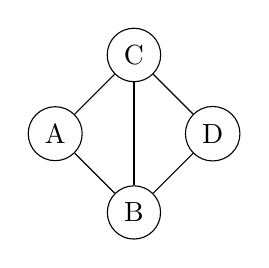
\begin{tikzpicture}[scale=1, every node/.style={circle, draw, fill=white, minimum size=6pt}]
  \node (A) at (0,1) {A};
  \node (B) at (1,0) {B};
  \node (C) at (1,2) {C};
  \node (D) at (2,1) {D};

  \draw (A) -- (B);
  \draw (A) -- (C);
  \draw (B) -- (D);
  \draw (C) -- (D);
  \draw (B) -- (C);
\end{tikzpicture}
\end{center}

Uno de ellos es el camino \( C \to A \to B \to D \to C \to B \).

\medskip

Sin embargo, este grafo \textbf{no} admite ningún circuito euleriano, ya que no es posible recorrer todas sus aristas y regresar al vértice de origen sin repetir alguna.
\end{exampleblock}

\begin{thmblock}{Caracterización de caminos eulerianos}
Sea \( G \) un multigrafo conexo con al menos dos vértices. Entonces \( G \) tiene un camino euleriano (pero no un circuito) si y sólo si tiene exactamente \textbf{dos vértices de grado impar}.
\end{thmblock}

\begin{proof}
\leavevmode
\begin{itemize}
\item[$\Rightarrow$] Sean \( u \) y \( v \) los extremos del camino euleriano. Como el camino recorre todas las aristas, debe contener todos los vértices del grafo. Para cualquier vértice intermedio \( t \), cada vez que se entra a \( t \), también se debe salir, lo que implica que su grado es par. Los extremos \( u \) y \( v \), en cambio, tienen grado impar, ya que sólo se entra o se sale una única vez más que el resto de las veces. Por lo tanto, \( G \) tiene exactamente dos vértices de grado impar.

\item[$\Leftarrow$] Supongamos ahora que \( G \) tiene exactamente dos vértices de grado impar, digamos \( u \) y \( v \). Construimos un nuevo grafo \( G' \) añadiendo una arista artificial entre \( u \) y \( v \). Este nuevo grafo \( G' \) tiene todos los vértices de grado par y es conexo, por lo que admite un circuito euleriano. Al eliminar la arista artificial, obtenemos un camino euleriano en \( G \) que comienza en \( u \) y termina en \( v \).
\end{itemize}
\end{proof}

\subsection{Caminos y circuitos eulerianos en grafos dirigidos}

En el caso de los grafos dirigidos, las condiciones para la existencia de un camino o circuito euleriano cambian ligeramente respecto del caso no dirigido.

\begin{thmblock}{Caracterización en grafos dirigidos}
Sea \( G \) un multigrafo dirigido sin vértices aislados.

\begin{itemize}
  \item \( G \) contiene un \textbf{circuito euleriano} si y sólo si:
  \begin{itemize}
    \item Es \textbf{débilmente conexo}, y
    \item El grado de entrada coincide con el grado de salida en cada vértice.
  \end{itemize}

  \item \( G \) contiene un \textbf{camino euleriano} (pero no un circuito) si y sólo si:
  \begin{itemize}
    \item Es \textbf{débilmente conexo}, y
    \item Todos los vértices tienen el mismo grado de entrada y de salida, excepto dos vértices \(v_1\) y \(v_2\), tales que:
    \[
    \degin{v_1} = \degout{v_1} + 1 \quad \text{y} \quad \degout{v_2} = \degin{v_2} + 1.
    \]
  \end{itemize}
\end{itemize}
\end{thmblock}

\medskip 
Notar que la existencia de un \textbf{circuito euleriano} en un grafo dirigido no implica que el grafo sea \emph{fuertemente conexo}.
En la Figura~\ref{fig:euleriano-no-fuerte}, el grafo tiene un circuito que recorre todas las aristas exactamente una vez, pero no existe camino dirigido entre algunos pares de vértices (por ejemplo, de \(C\) a \(A\)), por lo tanto no es fuertemente conexo.


\begin{figure}[ht]
\centering
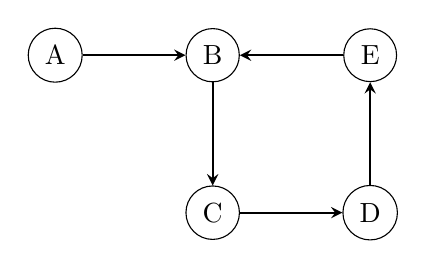
\begin{tikzpicture}[scale=1.0,
    every node/.style={circle, draw, fill=white, minimum size=7pt},
    arrow/.style={->, >=stealth, thick}
]

% Posiciones de los nodos
\node (A) at (0,1) {A};
\node (B) at (2,1) {B};
\node (C) at (2,-1) {C};
\node (D) at (4,-1) {D};
\node (E) at (4,1) {E};

% Flechas
\draw[arrow] (A) -- (B);
\draw[arrow] (B) -- (C);
\draw[arrow] (C) -- (D);
\draw[arrow] (D) -- (E);
\draw[arrow] (E) -- (B);
% \draw[arrow] (B) -- (A);

\end{tikzpicture}
\caption{Grafo dirigido con circuito euleriano \(A \rightarrow B \rightarrow C \rightarrow D \rightarrow E \rightarrow B \), pero que no es fuertemente conexo (por ejemplo, no hay camino dirigido de \(C\) a \(A\)).}
\label{fig:euleriano-no-fuerte}
\end{figure}




\section{Circuitos Hamiltonianos}

\subsection{Introducción}

Hasta ahora hemos estudiado los \textbf{circuitos eulerianos}, recorridos que atraviesan todas las \emph{aristas} de un grafo exactamente una vez. Esto es útil para problemas donde lo importante es cubrir todas las conexiones, como por ejemplo: Inspeccionar todos los cables de una red eléctrica.



En contraste, en muchas aplicaciones lo que se desea es visitar cada \textbf{vértice} exactamente una vez, sin repetir lugares:

\begin{itemize}
  \item Un viajante que quiere visitar cada ciudad una vez y volver al punto de origen,
  \item Un robot que debe recorrer todas las ubicaciones de una bodega sin repetir ninguna,
  \item Problemas de planificación o exploración sin retrocesos.
\end{itemize}


Este tipo de problema da origen a la noción de \textbf{circuito hamiltoniano}, llamado así en honor a William Rowan Hamilton, quien lo introdujo en el siglo XIX al estudiar recorridos sobre los vértices de un dodecaedro (poliedro de doce caras).

\begin{center}
\textit{¿Cuándo es posible visitar todos los vértices de un grafo sin repetir ninguno y volver al origen?}
\end{center}

\medskip

En esta sección exploraremos esta pregunta y veremos cómo, a diferencia del caso euleriano, determinar la existencia de un circuito hamiltoniano es un problema mucho más difícil, sin caracterización general conocida hasta la fecha.



\subsection{Definición}

\begin{definitionblock}{Circuito hamiltoniano}
Sea \( G \) un grafo. Un circuito de \( G \) se dice que es \textbf{hamiltoniano} si es simple y pasa por cada vértice de \( G \) exactamente una vez.
\end{definitionblock}

\begin{exampleblock}{Ejemplo}
Los siguientes grafos admiten un circuito hamiltoniano:

\medskip

\begin{center}
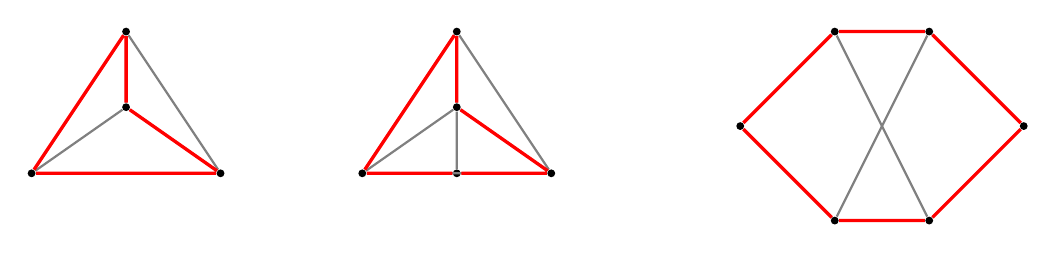
\begin{tikzpicture}[scale=1.2,
    every node/.style={circle, fill=black, inner sep=1pt},
    normal/.style={draw=gray, thick},
    highlight/.style={draw=red, very thick}
]

% -------- Primer grafo (triángulo con vértice interior) --------
\node (a1) at (0,0) {};
\node (a2) at (1,1.5) {};
\node (a3) at (2,0) {};
\node (a4) at (1,0.7) {}; % vértice interior

\draw[normal] (a1) -- (a2) -- (a3) -- (a1);
\draw[normal] (a2) -- (a4);
\draw[normal] (a3) -- (a4);
\draw[normal] (a1) -- (a4);

% Camino hamiltoniano (en rojo)
\draw[highlight] (a1) -- (a2) -- (a4) -- (a3) -- (a1);

% -------- Segundo grafo (doble triángulo conectado) --------
\begin{scope}[shift={(3.5,0)}]
\node (b1) at (0,0) {};
\node (b2) at (1,1.5) {};
\node (b3) at (2,0) {};
\node (b4) at (1,0.7) {};
\node (b5) at (1,0) {};

\draw[normal] (b1) -- (b2) -- (b3) -- (b1);
\draw[normal] (b1) -- (b4) -- (b3);
\draw[normal] (b2) -- (b4);
\draw[normal] (b4) -- (b5);
\draw[normal] (b1) -- (b5);
\draw[normal] (b3) -- (b5);

% Camino hamiltoniano
\draw[highlight] (b1) -- (b2) -- (b4) -- (b3) -- (b5) -- (b1) ;
\end{scope}

% -------- Tercer grafo (cuadrado con rombo interno) --------
\begin{scope}[shift={(7.5,0.5)}]
\node (A) at (0,0) {};
\node (B) at (1,1) {};
\node (C) at (2,1) {};
\node (D) at (3,0) {};
\node (E) at (2,-1) {};
\node (F) at (1,-1) {};

% Aristas de estructura
\draw[normal] (A) -- (B);
\draw[normal] (B) -- (C);
\draw[normal] (C) -- (D);
\draw[normal] (D) -- (E);
\draw[normal] (E) -- (F);
\draw[normal] (F) -- (A);
\draw[normal] (B) -- (E); % diagonales extra
\draw[normal] (C) -- (F);

% Camino hamiltoniano en rojo: A → B → C → D → E → F
\draw[highlight] (A) -- (B) -- (C) -- (D) -- (E) -- (F) -- (A) ;
\end{scope}
\end{tikzpicture}
\end{center}
\end{exampleblock}


A diferencia de los circuitos eulerianos, \textbf{no se conoce una caracterización eficiente} que permita determinar en general si un grafo tiene o no un circuito hamiltoniano.


\subsection{Condiciones necesarias y suficientes}

No existe una caracterización completa de los grafos que admiten circuitos hamiltonianos. Sin embargo, se conocen algunas condiciones útiles:

\begin{itemize}
  \item \textbf{Condiciones necesarias:} permiten descartar la existencia de un circuito hamiltoniano en algunos casos.
  \item \textbf{Condiciones suficientes:} garantizan su existencia en clases específicas de grafos (ver, por ejemplo, el teorema de Dirac y Ore).
\end{itemize}

\subsubsection{Condiciones necesarias para descartar hamiltonicidad}

Las siguientes observaciones permiten probar que un grafo \textbf{no} tiene circuitos hamiltonianos:

\begin{itemize}
  \item Si un grafo tiene un vértice de grado 1, no puede tener un circuito hamiltoniano.
  \item Si un vértice tiene grado 2, entonces \textbf{ambas aristas} incidentes deben formar parte de cualquier circuito hamiltoniano.
  \item Si un vértice tiene grado mayor a 2, y se sabe que \textbf{dos de sus aristas} están en un circuito hamiltoniano, entonces el \textbf{resto de las aristas incidentes no pueden estar} en dicho circuito.
\end{itemize}

% \subsection{Ejercicio: demostración por contradicción}

\begin{exampleblock}{Ejercicio: demostración por contradicción}
Utilice las condiciones anteriores para demostrar que los siguientes grafos \textbf{no} tienen circuitos hamiltonianos:

\begin{center}
\begin{tikzpicture}[scale=0.8,
  every node/.style={circle, fill=black, inner sep=1pt},
  label distance=2pt,
  font=\small
]

% -------- Grafo G (izquierda) --------
\node[label=above:$a$] (a) at (0,2) {};
\node[label=below:$b$] (b) at (0,0) {};
\node[label=below:$c$] (c) at (2,0) {};
\node[label=above:$d$] (d) at (2,2) {};
\node[label=above:$e$] (e) at (4,2) {};

% Aristas de G
\draw (a) -- (b);
\draw (a) -- (d);
\draw (b) -- (c);
\draw (c) -- (d);
\draw (d) -- (e);

% Nombre del grafo G
\node[draw=none, fill=none, font=\bfseries] at (2,-1) {$G$};

% -------- Grafo H (derecha) --------
\begin{scope}[shift={(7,0)}]
  \node[label=above:$a$] (a) at (0,2) {};
  \node[label=below:$b$] (b) at (0,0) {};
  \node[label=above:$d$] (d) at (3,2) {};
  \node[label=below:$e$] (e) at (3,0) {};
  \node[label=above :$c$] (c) at (1.5,1) {};

  \draw (a) -- (c);
  \draw (a) -- (b);
  \draw (b) -- (c);
  \draw (c) -- (d);
  \draw (c) -- (e);
  \draw (d) -- (e);

  % Nombre del grafo H
  \node[draw=none, fill=none, font=\bfseries] at (1.5,-1) {$H$};
\end{scope}

\end{tikzpicture}
\end{center}

\end{exampleblock}

\textbf{Solución:}

\begin{itemize}
  \item El grafo \( G \) no tiene circuito hamiltoniano porque contiene un vértice de grado 1.
  \item Para el grafo \( H \), supongamos por contradicción que tiene un circuito hamiltoniano. Como los vértices \( a, b, d, e \) tienen grado 2, las dos aristas incidentes en cada uno deben pertenecer al circuito. Por lo tanto, las 4 aristas que inciden en el vértice \( c \) también deberían pertenecer al circuito, lo cual es imposible (ya que solo puede tener 2 aristas en un camino simple cerrado). Esto contradice la tercera observación.
\end{itemize}


\subsubsection{Condiciones suficientes para circuitos hamiltonianos}

A diferencia de los circuitos eulerianos, no existe una caracterización general y eficiente que determine cuándo un grafo posee un circuito hamiltoniano. Sin embargo, existen ciertos resultados clásicos que establecen \textbf{condiciones suficientes} para garantizar su existencia.

\medskip

A continuación presentamos dos de los más conocidos: el \textbf{Teorema de Ore} y el \textbf{Teorema de Dirac}.


 Informalmente, si fijamos el conjunto de vértices de un grafo, en cuanto más
 artistas tenga, mayor potencial tendrá de contener caminos hamiltonianos.
 
El siguiente  teoremas establece que para que un grafo admita circuitos
hamiltonianos es condición suficiente que los vertices tengan grado ``lo
suficientemente grande''.


\begin{thmblock}{Teorema de Ore}
Sea \( G = (V,E) \) un grafo simple con \( n \geq 3 \) vértices.  
Si para todo par de vértices no adyacentes \( u, v \in V \) se cumple que
\[
\deg(u) + \deg(v) \geq n,
\]
entonces \( G \) posee un circuito hamiltoniano.
\end{thmblock}

Un corolario del Teorema de Ore, más simple de aplicar, es el siguiente:
\begin{thmblock}{Teorema de Dirac}
Sea \( G = (V,E) \) un grafo simple con \( n \geq 3 \) vértices.  
Si
\[
\deg(v) \geq \frac{n}{2} \quad \text{para todo } v \in V,
\]
entonces \( G \) posee un circuito hamiltoniano.
\end{thmblock}

\begin{proof}
El Teorema de Dirac es un caso particular del Teorema de Ore.  
En efecto, si todos los vértices tienen grado al menos \( \frac{n}{2} \), entonces para cualquier par de vértices no adyacentes \( u, v \),
\[
\deg(u) + \deg(v) \geq \frac{n}{2} + \frac{n}{2} = n,
\]
cumpliendo con la hipótesis del Teorema de Ore.
\end{proof}

\subsubsection{Ejercicios}

\begin{exampleblock}{Ejercicio}
Determinar cuáles de los siguientes grafos tienen un circuito hamiltoniano, justificando la respuesta:

\begin{center}
\begin{tikzpicture}[scale=1.0,
    every node/.style={circle, fill=black, inner sep=1pt},
    font=\footnotesize,
    label distance=2pt
]

% ---- Grafo 31 (izquierda) ----
\node[label=above:$a$] (a31) at (0,2) {};
\node[label=above:$b$] (b31) at (2,2) {};
\node[label=right:$c$] (c31) at (3,1) {};
\node[label=below:$d$] (d31) at (2,0) {};
\node[label=below:$e$] (e31) at (0,0) {};

% Aristas
\draw (a31) -- (b31);
\draw (a31) -- (e31);
\draw (e31) -- (d31);
\draw (b31) -- (d31);
\draw (b31) -- (c31);
\draw (d31) -- (c31);
\draw (b31) -- (e31);


% ---- Grafo 2 ----
\begin{scope}[shift={(6,0)}]
  \node[label=above:$a$] (a32) at (0,2) {};
  \node[label=above:$b$] (b32) at (2,2) {};
  \node[label=right:$c$] (c32) at (1,1) {};
  \node[label=below:$d$] (d32) at (0,0) {};
  \node[label=below:$e$] (e32) at (2,0) {};
  \node[label=below:$f$] (f32) at (3.5,0) {};

  % Aristas
  \draw (a32) -- (b32);
  \draw (a32) -- (c32);
  \draw (b32) -- (c32);
  \draw (c32) -- (e32);
  \draw (d32) -- (a32);
  \draw (d32) -- (e32);
  \draw (e32) -- (f32);
  \draw (b32) -- (e32);
\end{scope}

% ---- Grafo 3 ----
\begin{scope}[shift={(12,0)}]
  % Vértices izquierda
\node[label=above:$a$] (a) at (0,2) {};
\node[label=below:$b$] (b) at (0,0) {};
\node[label=above:$c$] (c) at (1,1) {};

% Vértices derecha
\node[label=above:$d$] (d) at (3,2) {};
\node[label=below:$e$] (e) at (3,0) {};
\node[label=above:$f$] (f) at (2,1) {};

% Aristas
\draw (a) -- (b);
\draw (a) -- (c);
\draw (b) -- (c);
\draw (d) -- (e);
\draw (d) -- (f);
\draw (e) -- (f);
\draw (c) -- (f);

\end{scope}

\end{tikzpicture}
\end{center}
\end{exampleblock}


\begin{exampleblock}{Ejercicio: grafo bipartito}
Sea \( K_{m,n} \) el grafo bipartito completo con \( m,n \geq 2 \).  
Probar que \( K_{m,n} \) tiene un circuito hamiltoniano si y sólo si \( m = n \).

\textbf{Hint:}
\begin{itemize}
  \item Para el \( \Rightarrow \): usar reducción al absurdo, suponiendo \( m \neq n \).
  \item Para el \( \Leftarrow \): aplicar el Teorema de Dirac.
\end{itemize}
\end{exampleblock}

\begin{proof}
\leavevmode
\begin{itemize}
\item[$\Rightarrow$]
Supongamos que \( K_{m,n} \) tiene un circuito hamiltoniano y que \( m \neq n \).  
Sin pérdida de generalidad, supongamos que \( m < n \). Sea \( A \) y \( B \) la partición del conjunto de vértices con \( |A| = m \) y \( |B| = n \), y supongamos que el recorrido parte desde \( a_1 \in A \).  
Como el grafo es bipartito, el circuito debe alternar entre vértices de \( A \) y \( B \).  
Luego de \( 2m \) pasos, se han recorrido todos los vértices de \( A \) y vuelto a \( a_1 \), pero aún quedarían \( n - m > 0 \) vértices en \( B \) sin visitar.  
Esto contradice que el recorrido sea hamiltoniano.

\item[$\Leftarrow$]
Si \( m = n \), entonces el grafo tiene \( 2m \) vértices y cada vértice tiene grado \( m \), cumpliendo:
\[
\deg(v) = m \geq \frac{2m}{2} = m.
\]
Por el Teorema de Dirac, \( K_{m,m} \) posee un circuito hamiltoniano.
\end{itemize}
\end{proof}